\documentclass{article}
\usepackage[a4paper,margin=0.1 cm,portrait]{geometry}
\usepackage{graphicx}
\usepackage{caption}
\usepackage{subcaption}
\usepackage{float}
\usepackage{booktabs}
\usepackage{tabularx}
\usepackage{ragged2e}
\setlength{\tabcolsep}{0.00\textwidth}



\begin{document}
%\centering


\begin{center}
\centering
\begin{tabularx}{1\textwidth}{cc}

\includegraphics[trim = 0mm 0mm 0mm 0mm, clip,width=0.35\textwidth]{off-targetA}  & 
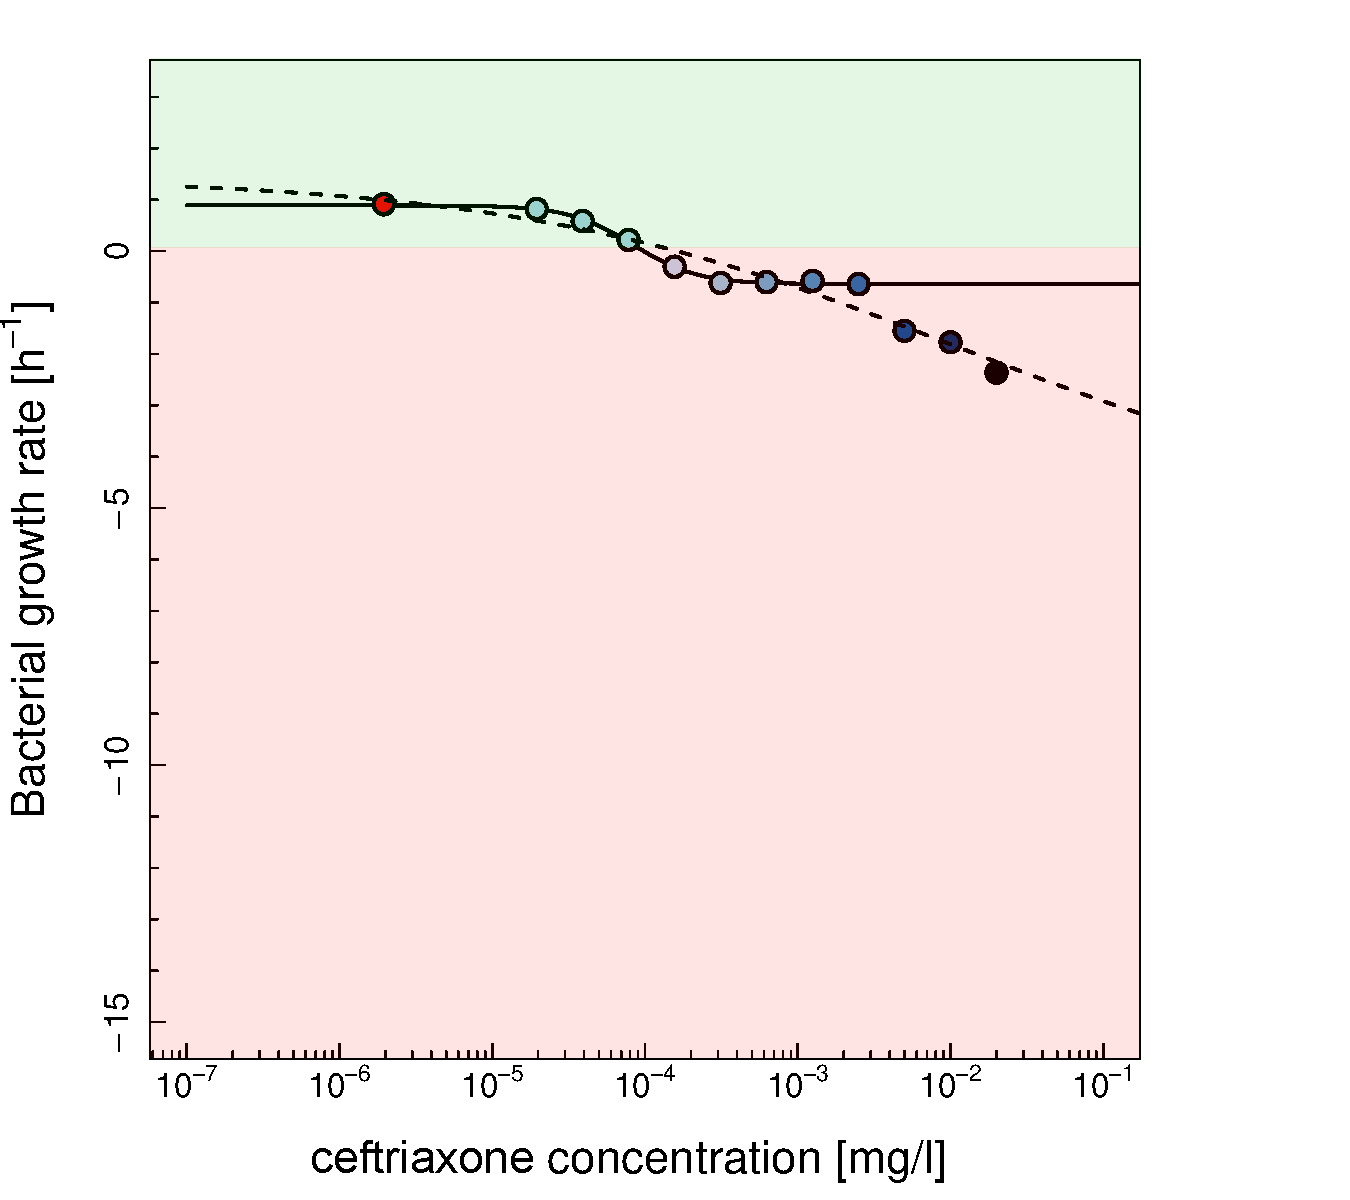
\includegraphics[trim = 0mm 0mm 0mm 0mm, clip,width=0.35\textwidth]{off-targetB}\\
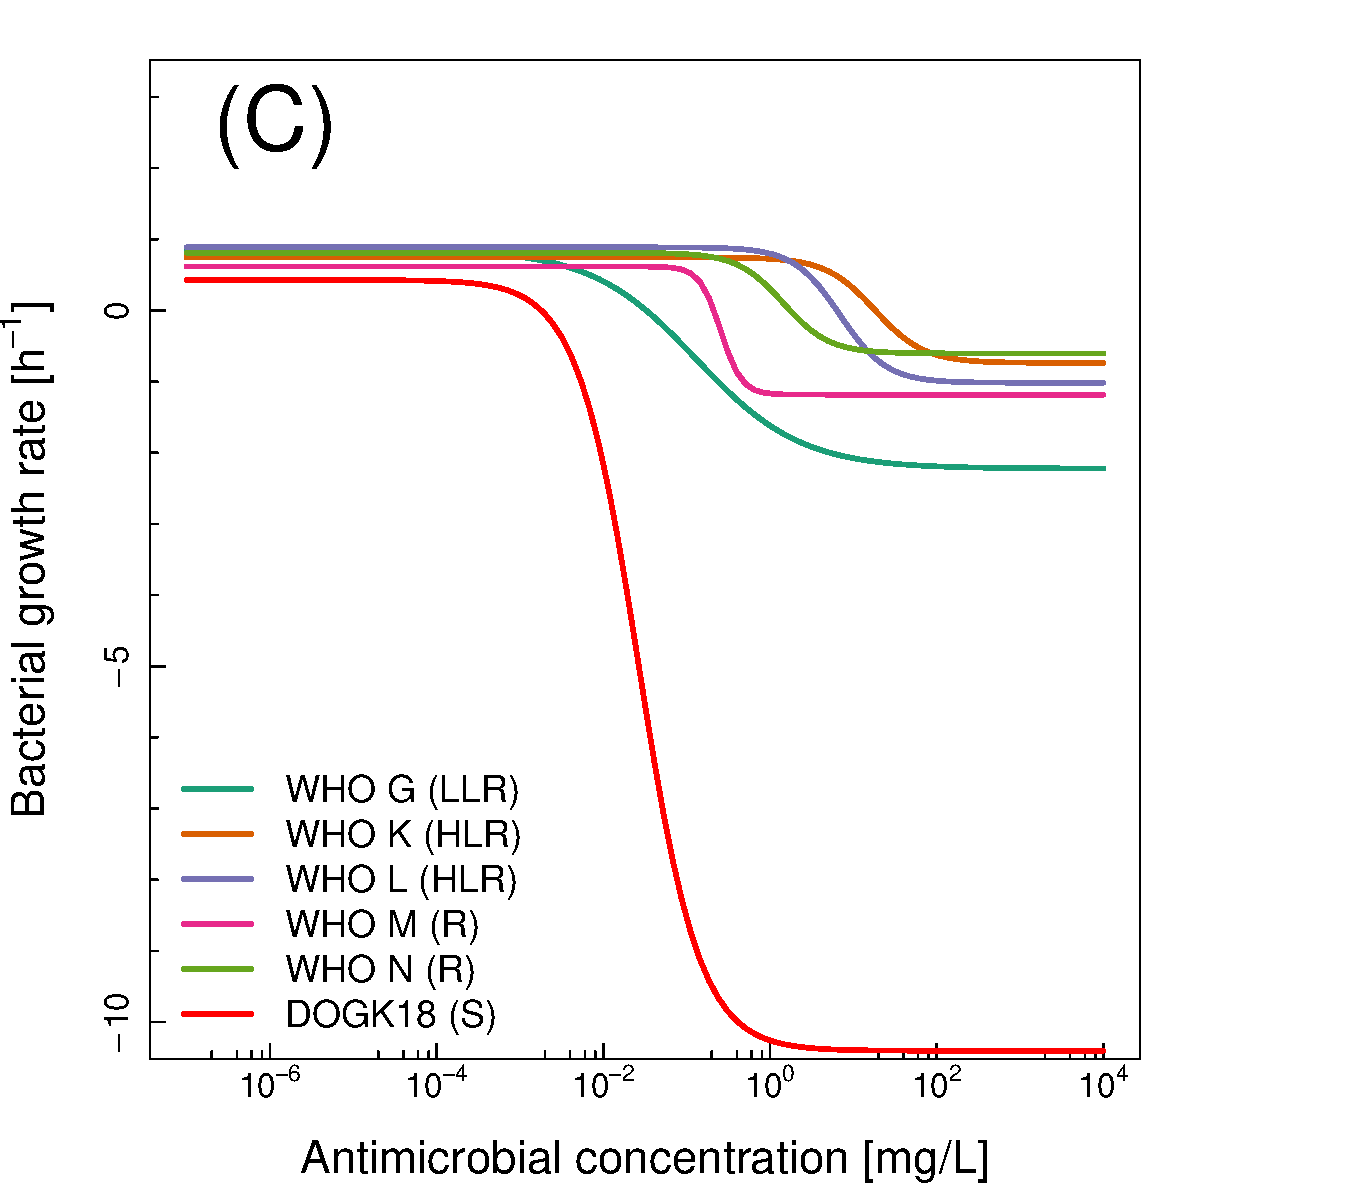
\includegraphics[trim = 0mm 0mm 0mm 0mm, clip,width=0.35\textwidth]{figure4C}&    
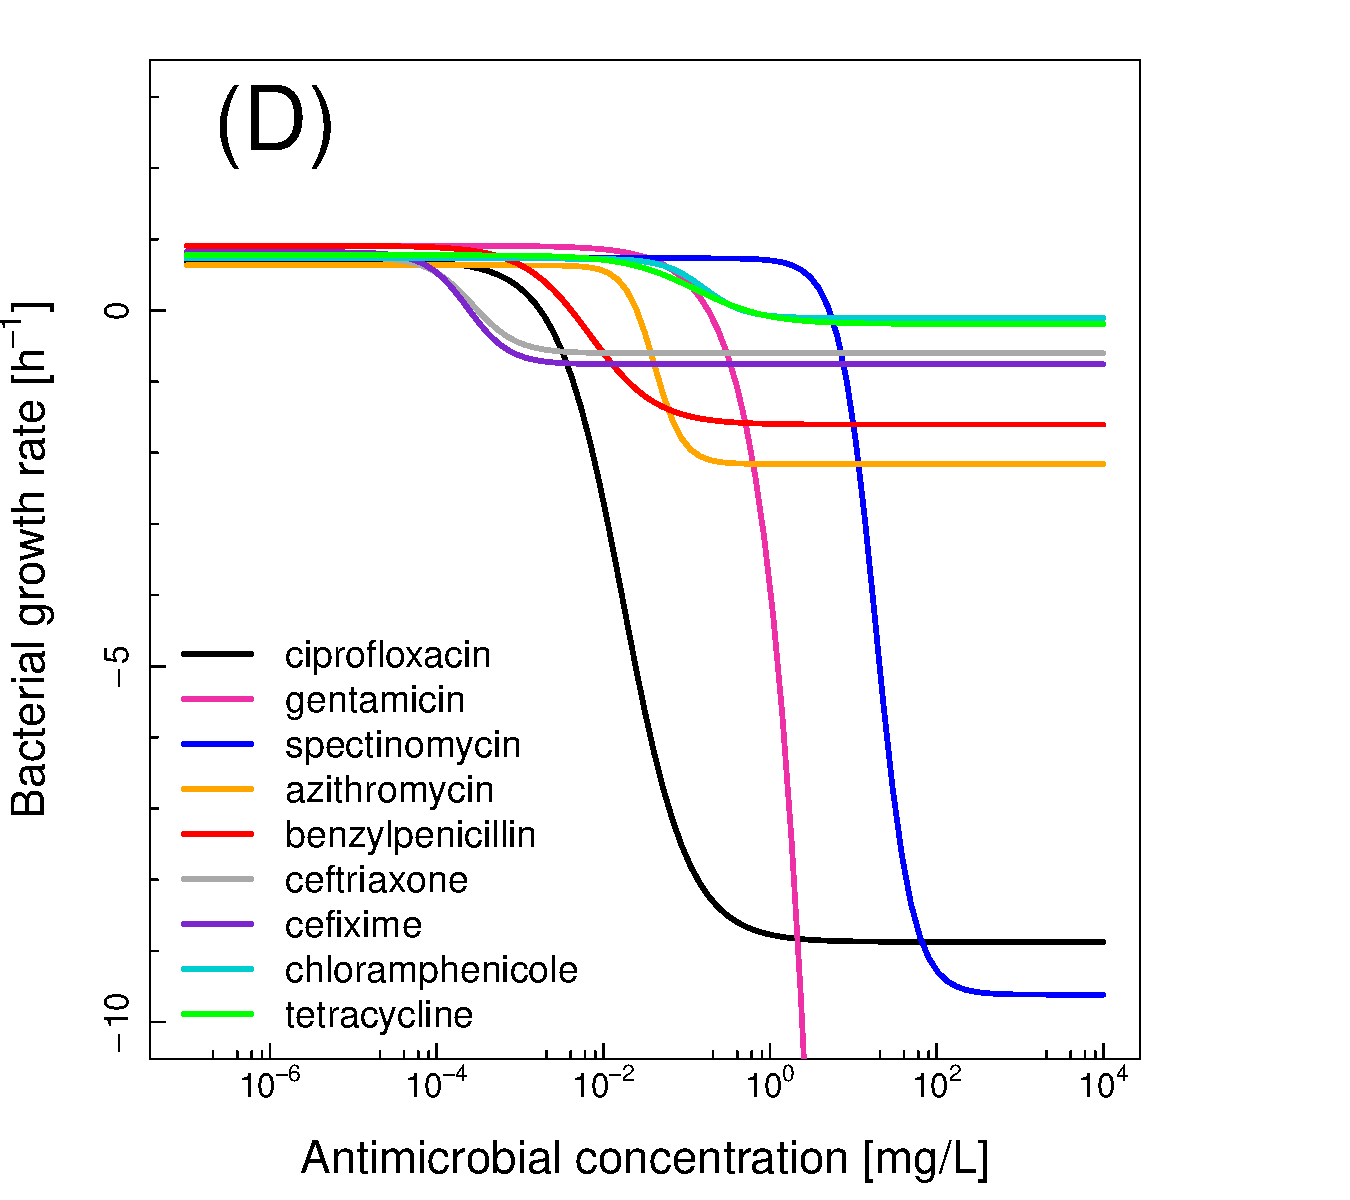
\includegraphics[trim = 0mm 0mm 0mm 0mm, clip,width=0.35\textwidth]{figure4D} \\ 
\end{tabularx}
\end{center}
\flushleft

\end{document}